%%%%%%%%%%%%%%%%%%%%%%%%%%%%%%%%%%%%%%%%%
% American Geophysical Union (AGU)
% LaTeX Template
% Version 1.0 (3/6/13)
%
% This template has been downloaded from:
% http://www.LaTeXTemplates.com
%
% Original author:
% The AGUTeX class and agu-ps referencing style were created and are owned 
% by AGU: http://publications.agu.org/author-resource-center/author-guide/latex-formatting-toolkit/
%
% This template has been modified from the blank AGU template to include
% examples of how to insert content and drastically change commenting. The
% structural integrity is maintained as in the original blank template.
%
% Important notes: 
% This template retains extensive commenting from the AGU template. It is heavily 
% advised you read these comments and follow them in order to insure a speedy 
% submission process.
%
%%%%%%%%%%%%%%%%%%%%%%%%%%%%%%%%%%%%%%%%%

%%%%%%%%%%%%%%%%%%%%%%%%%%%%%%%%%%%%%%%%%%%%%%%%%%%%%%%%%%%%%%%%%%%%%%%%%%%%
% AGUtmpl.tex: this template file is for articles formatted with LaTeX2e,
% Modified March 2013
%
%
% PLEASE DO NOT USE YOUR OWN MACROS
% DO NOT USE \newcommand, \renewcommand, or \def.
%
% FOR FIGURES, DO NOT USE \psfrag or \subfigure.
%
%%%%%%%%%%%%%%%%%%%%%%%%%%%%%%%%%%%%%%%%%%%%%%%%%%%%%%%%%%%%%%%%%%%%%%%%%%%%
%
% All questions should be e-mailed to latex@agu.org.
%
%%%%%%%%%%%%%%%%%%%%%%%%%%%%%%%%%%%%%%%%%%%%%%%%%%%%%%%%%%%%%%%%%%%%%%%%%%%%

% Step 1: Set the \documentclass

% There are two options for article format: two column (default) and draft.

% PLEASE USE THE DRAFT OPTION TO SUBMIT YOUR PAPERS.
% The draft option produces double spaced output.


\documentclass[draft,jgrga]{agutex}

% To create numbered lines:

% If you don't already have lineno.sty, you can download it from http://www.ctan.org/tex-archive/macros/latex/contrib/ednotes/ (or search the internet for lineno.sty ctan), available at TeX Archive Network (CTAN). Take care that you always use the latest version.

% To activate the commands, uncomment \usepackage{lineno} and \linenumbers*[1]command, below:

%\usepackage{lineno}
%\linenumbers*[1]

%  To add line numbers to lines with equations:
%  \begin{linenomath*}
%  \begin{equation}
%  \end{equation}
%  \end{linenomath*}

%%%%%%%%%%%%%%%%%%%%%%%%%%%%%%%%%%%%%%%%%%%%%%%%%%%%%%%%%%%%%%%%%%%%%%%%%
% Figures and Tables

% DO NOT USE \psfrag or \subfigure commands.

%  Figures and tables should be placed AT THE END OF THE ARTICLE, after the references.

%  Uncomment the following command to include .eps files (comment out this line for draft format):
%\usepackage[dvips]{graphicx}
\usepackage{graphicx}

% Substitute one of the following for [dvips] above if you are using a different driver program and want to proof your illustrations on your machine:
% [xdvi], [dvipdf], [dvipsone], [dviwindo], [emtex], [dviwin],
% [pctexps],  [pctexwin],  [pctexhp],  [pctex32], [truetex], [tcidvi],
% [oztex], [textures]

%  Uncomment the following command to allow illustrations to print when using Draft:
\setkeys{Gin}{draft=false}

% See how to enter figures and tables at the end of the article, after references.

%----------------------------------------------------------------------------------------
%	RUNNING HEAD AND CORRESPONDING AUTHOR
%----------------------------------------------------------------------------------------

% Author names in capital letters:
\authorrunninghead{Lee}

%------------------------------------------------

% Shorter version of title entered in capital letters:
\titlerunninghead{GEOPH 677 Final Project}

%------------------------------------------------

% Corresponding author mailing address and e-mail address:
\authoraddr{}

%----------------------------------------------------------------------------------------

\begin{document}

%----------------------------------------------------------------------------------------
%	TITLE
%----------------------------------------------------------------------------------------

\title{Title of the article}

%----------------------------------------------------------------------------------------
%	AUTHORS AND AFFILIATIONS
%----------------------------------------------------------------------------------------

% Use \author{\altaffilmark{}} and \altaffiltext{}

% \altaffilmark will produce footnote; matching \altaffiltext will appear at bottom of page.

\authors{Rebekah Lee}


%----------------------------------------------------------------------------------------
%	ABSTRACT
%----------------------------------------------------------------------------------------

% Do NOT include any \begin...\end commands within the body of the abstract.

% \begin{article}

\section{Abstract}

Lorem ipsum dolor sit amet, consectetur adipiscing elit. Sed vehicula metus sapien. Suspendisse pulvinar, felis ut hendrerit aliquet, dui nisi bibendum erat, fermentum mattis enim nibh id arcu. Vestibulum ultrices eros sed odio tincidunt bibendum. Pellentesque fermentum ante vel nulla commodo fermentum. Vestibulum in augue sit amet libero viverra accumsan eu at magna. Sed at ligula quis nibh pharetra facilisis non eu libero. Suspendisse non quam sit amet massa luctus interdum sit amet in purus. Integer id orci elit, vitae sollicitudin lectus.


%----------------------------------------------------------------------------------------
%	ARTICLE CONTENT
%----------------------------------------------------------------------------------------

% The body of the article must start with a \begin{article} command
% \end{article} must follow the references section, before the figures and tables.


\section{Introduction}

Nam fermentum sapien at enim varius consectetur. Quisque lobortis imperdiet mauris, et accumsan libero vulputate vitae. Integer lacinia purus vel metus tempus suscipit. Curabitur ac sapien quis mauris euismod commodo. Sed pharetra sem elit. Fusce ultrices, mauris eu fermentum tempor, tellus sem ornare lectus, in convallis nunc urna id dolor. Donec convallis ligula vitae sem viverra fermentum. Mauris in ullamcorper erat. Donec ultrices tempus nibh quis vestibulum. This statement requires citation \citep{Goldfinger2013}. This one is an in-text citation because the authors of \citet{Herrendorfer2015} are specifically mentioned.

Praesent volutpat, nibh in dignissim commodo, tellus justo consequat erat, vel consequat mi arcu vel lectus. Aliquam a tellus nec felis sagittis consequat. Quisque convallis imperdiet neque a tempor. Nulla non erat urna. Mauris vel lorem magna, tristique auctor ipsum. Aliquam pharetra eleifend massa. Donec porttitor sagittis luctus. Aliquam pretium luctus leo quis congue. Morbi vel felis mi. Suspendisse viverra tortor pretium orci lacinia eleifend. Phasellus aliquam, nunc eu cursus feugiat, erat odio porttitor libero, quis accumsan orci ipsum ut lorem. Vestibulum pharetra malesuada egestas. Sed non orci sit amet erat suscipit fringilla in et diam. Vestibulum ante ipsum primis in faucibus orci luctus et ultrices posuere cubilia Curae; Nunc ut rhoncus nulla. Aenean porta rhoncus suscipit.

%------------------------------------------------
\newpage
\section{Methods}

\citet{Herrendorfer2015} model subduction zones using a two-dimensional numerical model of a simplified and scaled subduction zone to investigate the role of the seimogenic zone downdip width. In this model a rigid plate subducts beneath a visco-elastic wedge at an angle of $10^\circ$. The seismogenic zone has velocity weakening properties, whereas the aseismic zone has velocity strengthening properties. The authors use conservative finite differences to solve for conservation of mass (eq. \ref{eqn:mass}) and momentum (eq. \ref{eqn:momentum}) under the assumption of incompressibility ($\nabla \cdot \vec{v}$):
\begin{equation}
	\frac{\partial v_x}{\partial x} + \frac{\partial v_y}{\partial y} = 0,
	\label{eqn:mass}
\end{equation}
\begin{eqnarray}\hspace{5.8cm}
\frac{\partial \sigma'_{xx}}{\partial x} + \frac{\sigma'_{yy}}{\partial y} - \frac{\partial P}{\partial x} = \rho\frac{Dv_x}{Dt} \nonumber 
\end{eqnarray}

\begin{equation}
	\frac{\partial \sigma'_{yx}}{\partial x} + \frac{\sigma'_{yy}}{\partial y} - \frac{\partial P}{\partial y} = \rho\frac{Dv_y}{Dt} - \rho g
	\label{eqn:momentum}
\end{equation}
% \begin{equation}
%\frac{\partial \sigma'_{xx}}{\partial x} + \frac{\sigma'_{yy}}{\partial y} - \frac{\partial P}{\partial x} = \rho\frac{Dv_x}{Dt} \nonumber\\
	%\frac{\partial \sigma'_{yx}}{\partial x} + \frac{\sigma'_{yy}}{\partial y} - \frac{\partial P}{\partial y} = \rho\frac{Dv_y}{Dt} - \rho g 
	
% \end{equation}
where $v_x$ and $v_y$ are horizontal and vertical velocities, $\sigma'$ is the stress tensor, P is pressure, g is the gravitaional constant and $\rho$ is density. The authors use a constitutive relationship that connects the deviatoric stresses ($\sigma'_{ij}$) and strain rates ($\dot{\epsilon}'_{ij}$) applying linear elasticity and Newtonian viscosity: EQN4HERE

%\begin{equation}
	
%\end{equation}
where G is shear modulus, $\eta$ is effective viscosity, $\sigma'_{II} = \sqrt{\sigma'^2_{xx} + \sigma'^2_{xy}}$ is the plastic flow potential, and $\chi$ is a plastic multiplier connecting plastic strain rates and stresses.

Flow becomes plastic when the plastic flow potential, $\sigma'_{II}$ reaches the local pressure-dependent yield strength, $\sigma_{yield}$:

\begin{equation}
	 	\sigma'_{II} = \sigma_{yield} = C + \mu_{eff} \cdot P, 
 \end{equation} 
where C is cohesion and $\mu_{eff}$ is the effective friction coefficient. $\mu_{eff}$ is strongly rate dependent as it depends on the visco-plastic slip velocity, $V_{vp}$:
\begin{equation}
 	\mu_{eff} = \mu_s(1-\gamma) + \mu_s\frac{\gamma}{1 + \frac{V_{vp}}{V_c}},
 \end{equation} 
 where  $\gamma$ is amount of weakening ($1 - \frac{\mu_s}{\mu_d}$), $\mu_s$ and $\mu_d$ are static and dynamic coefficients, respectively, and $V_c$ is characteristic slip velocity. 

During plastic deformation elastic strain is zero and the second invariant of deviatoric stresses must be constant. The total strain rate therefore is the sum of the viscous and plastic strain rates, so that the plastic strain is $\dot{\epsilon}'_{II} - \dot{\epsilon}'^{(viscous)}_{II}$ (where $\dot{\epsilon}'_{II} = \sqrt{\dot{\epsilon}'^2_{xx} + \dot{\epsilon}'^2_{xy}}$ ) and the visco-plastic viscosity is:
\begin{equation}
 	\eta_{vp} = \eta\frac{\sigma'_{II}}{\eta\chi + \sigma'_{II}},
 \end{equation} 
with 
\begin{equation}
	\chi = 2(\dot{\epsilon}'_{II} - \dot{\epsilon}'^{(viscous)}_{II}) = 2(\dot{\epsilon}'_{II} - \frac{1}{2\eta}\sigma'_{II})
\end{equation}

 The authors define subcritical ruptures as events that fail to propagate a long distance out of their nucleation region. Pulse-like ruptures propagate further than subcritical ruptures but have a local duration of coseismic displacements that is short compared to the total rupture duration. In a crack-like rupture most of the rupture area continues to slip until the end of the rupture. See column three of figure \ref{fig:ruptureStyle} for plots of the horizontal velocity through time and distance from backstop for each of the rupture types.


%-----------------------------------------------------------------------------------------------------------
%									Data and Results
%-----------------------------------------------------------------------------------------------------------
\section{Data and Results}
The tsunami record near Sendai, Japan shows events in 1896, 1611 and 869. The largest is the 869 even with tsunami penetrating $3-4$ km inland, similar to the 2011 earthquake. There is also evidence for two predecessors with tsunamis reaching the same distance inland as the 869 and 2011 earthquakes. This evidence supports the existence of periodic outsized earthquakes greater than magnitude 9 with a recurrance interval between $800 -1200$ years \citep{Goldfinger2013}.

\begin{figure}
% \hspace{-1cm}
	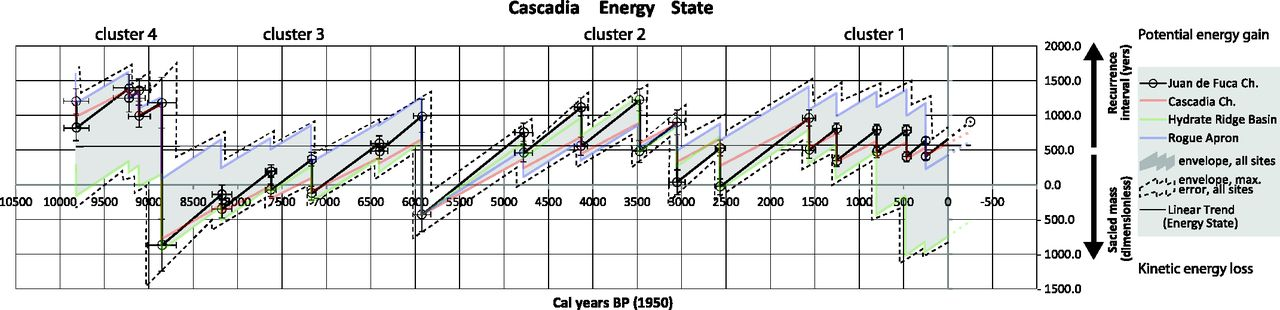
\includegraphics[width=1\linewidth]{./Figures/Goldfinger/F4large.jpg}
	\caption{caption here}
	\label{fig:energyCycle}
\end{figure}


\citet{Goldfinger2013} identify the Cascadia subduction zone as another area likely to produce supercycle earthquakes. They correlate turbidite cores along the subduction zone and find consistency between sites for the same events in terms of mass size. 

Figure {\bf \ref{fig:energyCycle}} shows the results from modeling the energy state in the Cascadia subduction zone \citep{Goldfinger2013}. 

They identify four clusters from the past 10 thousand years. Cluster four shows an even energy state before falling to a low after a large event. Cluster 3 climbs steadily until falling to a similar low. During this period there are several seismic cycles with relatively low stress drops that do not relieve all of the accumulated strain. A total stress drop finally happens at the end of the cluster with an event much larger than the others within the same cluster. Cluster two differs from the previous in that it does not culminate in an oversized event. Rather, it climbs and then falls over several seismic cycles until it reaches a low energy value about 2500 years BP (1950). The end of the cluster marks a long gap of about 1,000 years of constant increase in energy. Cluster one then slowly decreases the energy state until the A.D. 1700 $M_w$ ~9.0 earthquake. \citep{Goldfinger2013} note that the scale factor is based on the condition of no net energy change over the 10,000 years but that changing this parameter does not change the pattern observed. The authors also note that the seismic coupling coefficient only changes the pattern if the value is allowed to vary between events. 

The four clusters modeled by \citet{Goldfinger2013} demonstrate that some events in this subduction zone release energy from previous cycles. This subduction zone is neither slip nor time predictable. Energy release is not tied to recurrance intervals as some events can release energy accumulated from previous seismic cycles. The authors make a few observations relating the energy state to the behavior of the clusters. High energy states results in one very large event, (as in the case of cluster four), or a series of smaller events (as in cluster two). Low energy state results in a long gap in seismicity (cluster 2) or a series of small earthquakes with net energy gain over several cycles (cluster 3). 

\begin{figure}
	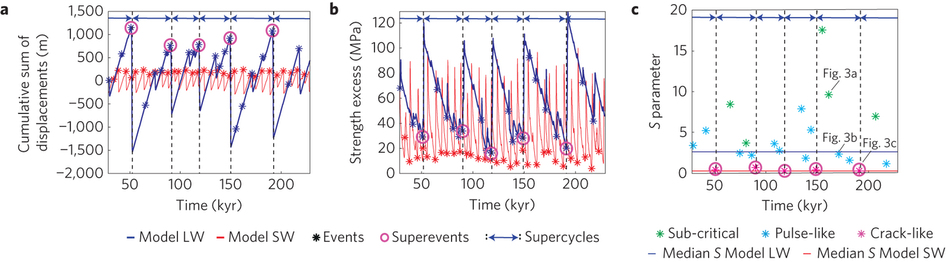
\includegraphics[width=1\linewidth]{Figures/Herrendorfer/ngeo2427-f2.jpeg}
	\caption{Comparison of characteristics of long (LW) and small (SW) downdip width subduction zone models. Earthquakes indicated by astericks and superevents are circled. Subfigures show cumulative sum over time ({\bf a}) Excess strength ({\bf b}) and S parameter ({\bf b}). S parameter is the ratio of initial strength excess to stress change during an event. Event types are also indicated by color. From \citet{Herrendorfer2015}.}
	\label{fig:SZOwidth}
\end{figure}
\begin{figure}
	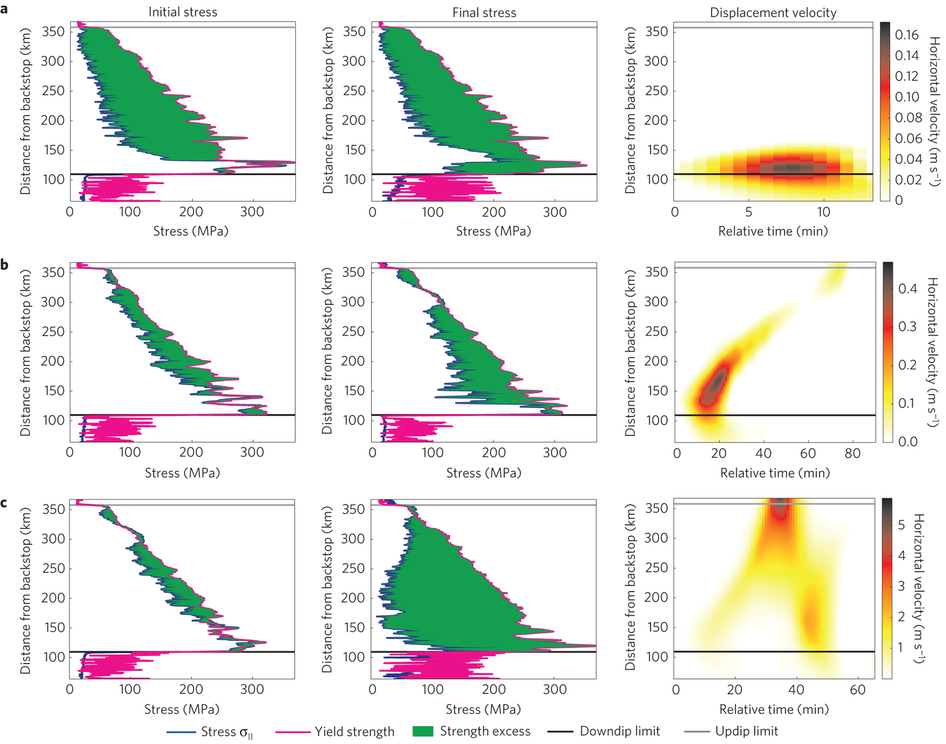
\includegraphics[width=1\linewidth]{Figures/Herrendorfer/ngeo2427-f3.jpeg}
	\caption{caption}
	\label{fig:ruptureStyle}
\end{figure}

Figures {\bf \ref{fig:SZOwidth},\ref{fig:ruptureStyle}} show results from \citet{Herrendorfer2015}. Both systems show that events are triggered at low excess stress (Figure {\bf \ref{fig:SZOwidth}b}). However, the magnitudes at similar low stresses are much greater for the large width subduction zone, as shown in Figure ({\bf \ref{fig:SZOwidth}a}). Large width zones are characterized by supercycles that partially release stress but overall excess strength continues to decrease until at a low level. Figure {\bf \ref{fig:ruptureStyle}} shows strength excess (shaded green) before and after each of the event types. Subcritical events (a) nucleate close to the downdip limit of the seismogenic zone and transfers stress close to the stopping location (about 125 km from backstop). Pulse-like ruptures (b) nucleate from the downdip limit for short duration and transfer stress updip (about 300 km from backstop). These combine to shift the strain towards the center of the seismogenic zone that eventually results in the crack-like event (c) that ruptures the entire zone. 

\citet{Herrendorfer2015} characterize events by an S parameter. The S parameter is a measure of the ratio the inital strength excess and stress change during an event. Figure {\bf \ref{fig:SZOwidth}} Large width model is characterized by a higher median S parameter (2.5) compared to the small width model (.25). The average strength excess is increased by increased width and leads to transition from crack-like ruptures of the entire zone to smaller preparatory subcritical and pulse-like ruptures leading up to culminating crack-like rupture. 

%------------------------------------------------

\section{Conclusion}
Examining the geologic record can give us a good indication of whether or not a subduction zone has produced oversized events in the past. This records include paleoseimic eveidence and tsunami observations and turbidite deposits when they can be attributed to shaking. As the data from the Cascadias demonstrates, there is no simply relationship to predict the size of earthquakes in subduction zones. For example, because supercycles use energy from previous seismic cycles, convergent rate is an unreliable predictor as some earthquakes may not result in a complete stress drop over the area of the fault. 






%----------------------------------------------------------------------------------------
%	BIBLIOGRAPHY
%----------------------------------------------------------------------------------------

% Either type in your references using
% \begin{thebibliography}{}
% \bibitem{}
% Text
% \end{thebibliography}

% Or,

% If you use BiBTeX for your references, please use the agufull08.bst file (available at % ftp://ftp.agu.org/journals/latex/journals/Manuscript-Preparation/) to produce your .bbl
% file and copy the contents into your paper here.

% Follow these steps:
% 1. Run LaTeX on your LaTeX file.

% 2. Make sure the bibliography style appears as \bibliographystyle{agufull08}. Run BiBTeX on your LaTeX
% file.

% 3. Open the new .bbl file containing the reference list and
%   copy all the contents into your LaTeX file here.

% 4. Comment out the old \bibliographystyle and \bibliography commands.

% 5. Run LaTeX on your new file before submitting.

% AGU does not want a .bib or a .bbl file. Please copy in the contents of your .bbl file here.



% Reference citation examples:

%...as shown by \textit{Kilby} [2008].
%...as shown by {\textit  {Lewin}} [1976], {\textit  {Carson}} [1986], {\textit  {Bartholdy and Billi}} [2002], and {\textit  {Rinaldi}} [2003].
%...has been shown [\textit{Kilby et al.}, 2008].
%...has been shown [{\textit  {Lewin}}, 1976; {\textit  {Carson}}, 1986; {\textit  {Bartholdy and Billi}}, 2002; {\textit  {Rinaldi}}, 2003].
%...has been shown [e.g., {\textit  {Lewin}}, 1976; {\textit  {Carson}}, 1986; {\textit  {Bartholdy and Billi}}, 2002; {\textit  {Rinaldi}}, 2003].

%...as shown by \citet{jskilby}.
%...as shown by \citet{lewin76}, \citet{carson86}, \citet{bartoldy02}, and \citet{rinaldi03}.
%...has been shown \citep{jskilbye}.
%...has been shown \citep{lewin76,carson86,bartoldy02,rinaldi03}.
%...has been shown \citep [e.g.,][]{lewin76,carson86,bartoldy02,rinaldi03}.

% Please use ONLY \citet and \citep for reference citations.
% DO NOT use other cite commands (e.g., \cite, \citeyear, \nocite, \citealp, etc.).

% \end{article}
\newpage
\bibliography{sources}
\bibliographystyle{agufull08}
%----------------------------------------------------------------------------------------
%	FIGURES AND TABLES
%----------------------------------------------------------------------------------------

%% Enter Figures and Tables here:
%
% DO NOT USE \psfrag or \subfigure commands.
%
% Figure captions go below the figure.
% Table titles go above tables; all other caption information should be placed in footnotes below the table.
%
%----------------
% EXAMPLE FIGURE
%
% \begin{figure}
% \noindent\includegraphics[width=20pc]{samplefigure.eps}
% \caption{Caption text here}
% \label{figure_label}
% \end{figure}
%
% ---------------
% EXAMPLE TABLE
%
%\begin{table}
%\caption{Time of the Transition Between Phase 1 and Phase 2\tablenotemark{a}}
%\centering
%\begin{tabular}{l c}
%\hline
% Run  & Time (min)  \\
%\hline
%  $l1$  & 260   \\
%  $l2$  & 300   \\
%  $l3$  & 340   \\
%  $h1$  & 270   \\
%  $h2$  & 250   \\
%  $h3$  & 380   \\
%  $r1$  & 370   \\
%  $r2$  & 390   \\
%\hline
%\end{tabular}
%\tablenotetext{a}{Footnote text here.}
%\end{table}

% See below for how to make sideways figures or tables.



\end{document}

%%%%%%%%%%%%%%%%%%%%%%%%%%%%%%%%%%%%%%%%%%%%%%%%%%%%%%%%%%%%%%%

More Information and Advice:

%% ------------------------------------------------------------------------ %%
%
%  SECTION HEADS
%
%% ------------------------------------------------------------------------ %%

% Capitalize the first letter of each word (except for
% prepositions, conjunctions, and articles that are
% three or fewer letters).

% AGU follows standard outline style; therefore, there cannot be a section 1 without
% a section 2, or a section 2.3.1 without a section 2.3.2.
% Please make sure your section numbers are balanced.
% ---------------
% Level 1 head
%
% Use the \section{} command to identify level 1 heads;
% type the appropriate head wording between the curly
% brackets, as shown below.
%
%An example:
%\section{Level 1 Head: Introduction}
%
% ---------------
% Level 2 head
%
% Use the \subsection{} command to identify level 2 heads.
%An example:
%\subsection{Level 2 Head}
%
% ---------------
% Level 3 head
%
% Use the \subsubsection{} command to identify level 3 heads
%An example:
%\subsubsection{Level 3 Head}
%
%---------------
% Level 4 head
%
% Use the \subsubsubsection{} command to identify level 3 heads
% An example:
%\subsubsubsection{Level 4 Head} An example.
%
%% ------------------------------------------------------------------------ %%
%
%  IN-TEXT LISTS
%
%% ------------------------------------------------------------------------ %%
%
% Do not use bulleted lists; enumerated lists are okay.
% \begin{enumerate}
% \item
% \item
% \item
% \end{enumerate}
%
%% ------------------------------------------------------------------------ %%
%
%  EQUATIONS
%
%% ------------------------------------------------------------------------ %%

% Single-line equations are centered.
% Equation arrays will appear left-aligned.

Math coded inside display math mode \[ ...\]
 will not be numbered, e.g.,:
 \[ x^2=y^2 + z^2\]

 Math coded inside \begin{equation} and \end{equation} will
 be automatically numbered, e.g.,:
 \begin{equation}
 x^2=y^2 + z^2
 \end{equation}

% IF YOU HAVE MULTI-LINE EQUATIONS, PLEASE
% BREAK THE EQUATIONS INTO TWO OR MORE LINES
% OF SINGLE COLUMN WIDTH (20 pc, 8.3 cm)
% using double backslashes (\\).

% To create multiline equations, use the
% \begin{eqnarray} and \end{eqnarray} environment
% as demonstrated below.
\begin{eqnarray}
  x_{1} & = & (x - x_{0}) \cos \Theta \nonumber \\
        && + (y - y_{0}) \sin \Theta  \nonumber \\
  y_{1} & = & -(x - x_{0}) \sin \Theta \nonumber \\
        && + (y - y_{0}) \cos \Theta.
\end{eqnarray}

%If you don't want an equation number, use the star form:
%\begin{eqnarray*}...\end{eqnarray*}

% Break each line at a sign of operation
% (+, -, etc.) if possible, with the sign of operation
% on the new line.

% Indent second and subsequent lines to align with the first character following the equal sign on the first line.

% Use an \hspace{} command to insert horizontal space into your equation if necessary. Place an appropriate unit of measure between the curly braces, e.g. \hspace{1in}; you may have to experiment to achieve the correct amount of space.


%% ------------------------------------------------------------------------ %%
%
%  EQUATION NUMBERING: COUNTER
%
%% ------------------------------------------------------------------------ %%

% You may change equation numbering by resetting
% the equation counter or by explicitly numbering
% an equation.

% To explicitly number an equation, type \eqnum{}
% (with the desired number between the brackets)
% after the \begin{equation} or \begin{eqnarray}
% command.  The \eqnum{} command will affect only
% the equation it appears with; LaTeX will number
% any equations appearing later in the manuscript
% according to the equation counter.
%

% If you have a multiline equation that needs only
% one equation number, use a \nonumber command in
% front of the double backslashes (\\) as shown in
% the multiline equation above.

%% ------------------------------------------------------------------------ %%
%
%  SIDEWAYS FIGURE AND TABLE EXAMPLES
%
%% ------------------------------------------------------------------------ %%
%
% For tables and figures, add \usepackage{rotating} to the paper and add the rotating.sty file to the folder.
% AGU prefers the use of {sidewaystable} over {landscapetable} as it causes fewer problems.
%
% \begin{sidewaysfigure}
% \includegraphics[width=20pc]{samplefigure.eps}
% \caption{caption here}
% \label{label_here}
% \end{sidewaysfigure}
%
% \begin{sidewaystable}
% \caption{}
% \begin{tabular}
% Table layout here.
% \end{tabular}
% \end{sidewaystable}